\documentclass{beamer}
\usetheme{Boadilla}

\usepackage{amsmath}
\usepackage{amsfonts}
\usepackage{hyperref}
\usepackage{biblatex}
\graphicspath{ {./images/} }


\title{Predictive Uncertainty Estimation via Prior Networks}
\author{Ksenofontov Gregory}
\institute{MIPT}


\begin{document}

\begin{frame}
    \titlepage
\end{frame}

\begin{frame}{Predictive uncertainty}
     \begin{enumerate}
        \item \textbf{Model uncertainty}, or \textbf{epistemic uncertainty}, measures how well the model (parameters) is matched to the data
        \item \textbf{Data uncertainty}, or \textbf{aleatoric uncertainty}, arises from the natural complexity of the data, such as class overlap, label noise. The model understands the data and can confidently state whether a given input is difficult to classify. 
        \item \textbf{Distributional uncertainty}, \textbf{dataset shift}, arises due to mismatch between the training and test distributions. The model is unfamiliar with the test data and thus cannot confidently make predictions. 
    \end{enumerate}
\end{frame}

\begin{frame}{Previous approaches}
\textbf{Bayesian class:} 
    \begin{enumerate}
        \item more complicated conceptually
        \item performance depends on the form of approximation and the nature of the prior distribution of parameters
        \item implicitly model distributional uncertainty through model uncertainty
    \end{enumerate}
    \textbf{Non-Bayesian class:}
    \begin{enumerate}
        \item more straight forward
        \item explicitly lowers uncertainty on training data and heighten uncertainty on generated artificial data
        \item conflate distributional uncertainty with data uncertainty
    \end{enumerate}
\end{frame}

\begin{frame}{Bayesian class}
     Consider a distribution $p(\mathbf{x}, y)$ over input features $\mathbf{x}$, labels $y$ and classification model $P(y = \omega_c | \mathbf{x}^*, \mathbf{\theta})$, trained on $D = \{\mathbf{x}_j, y_j\}_{j=1}^N \sim p(\mathbf{x}, y)$. So, in Bayesian framework the uncertainty is:
     $$P(\omega_c | \mathbf{x}^*, D) = \int P(\omega_c | \mathbf{x}^*, \mathbf{\theta})p(\mathbf{\theta}|D) d\mathbf{\theta}$$
     where $P(\omega_c | \mathbf{x}^*, \mathbf{\theta})$ - data uncertainty,
     $p(\mathbf{\theta}|D)$ - model uncertainty
     $$P(\omega_c | \mathbf{x}^*, D) \approx \frac{1}{M}\sum_{i=1}^MP(\omega_c | \mathbf{x}^*, \mathbf{\theta}^{(i)}), \mathbf{\theta}^{(i)} \sim q(\mathbf{\theta})$$
     \begin{figure}[h]
        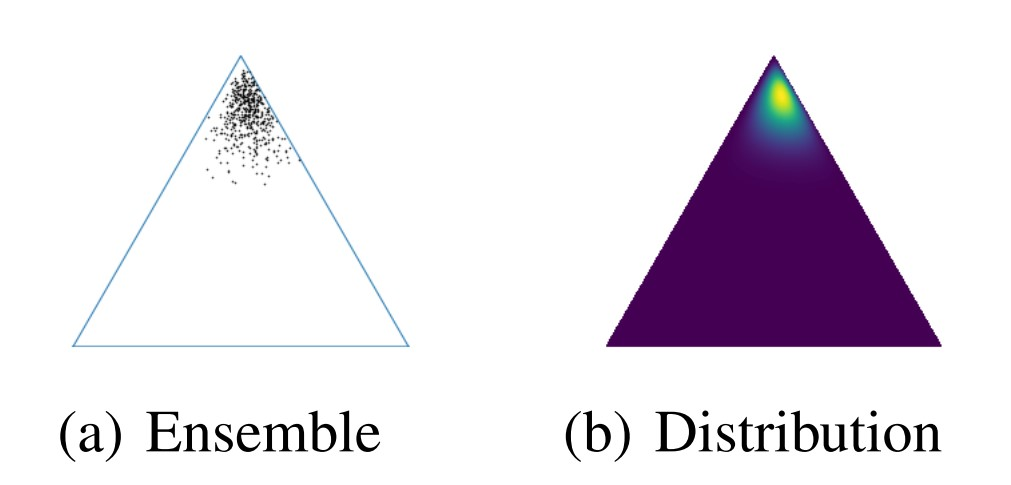
\includegraphics[scale=0.25]{ensamble.jpg}
     \end{figure}
\end{frame}


\begin{frame}{Prior Networks}
    $$P(\omega_c | \mathbf{x}^*, D) = \int \int p(\omega_c | \mathbf{\mu}) p(\mu | \mathbf{x}^*, \mathbf{\theta})p(\mathbf{\theta}|D) d\mathbf{\mu}d\mathbf{\theta}$$
    where $p(\omega_c | \mathbf{\mu})$ - data uncertainty,
    $p(\mu | \mathbf{x}^*, \mathbf{\theta})$ - distributional uncertainty
    \begin{figure}[h]
        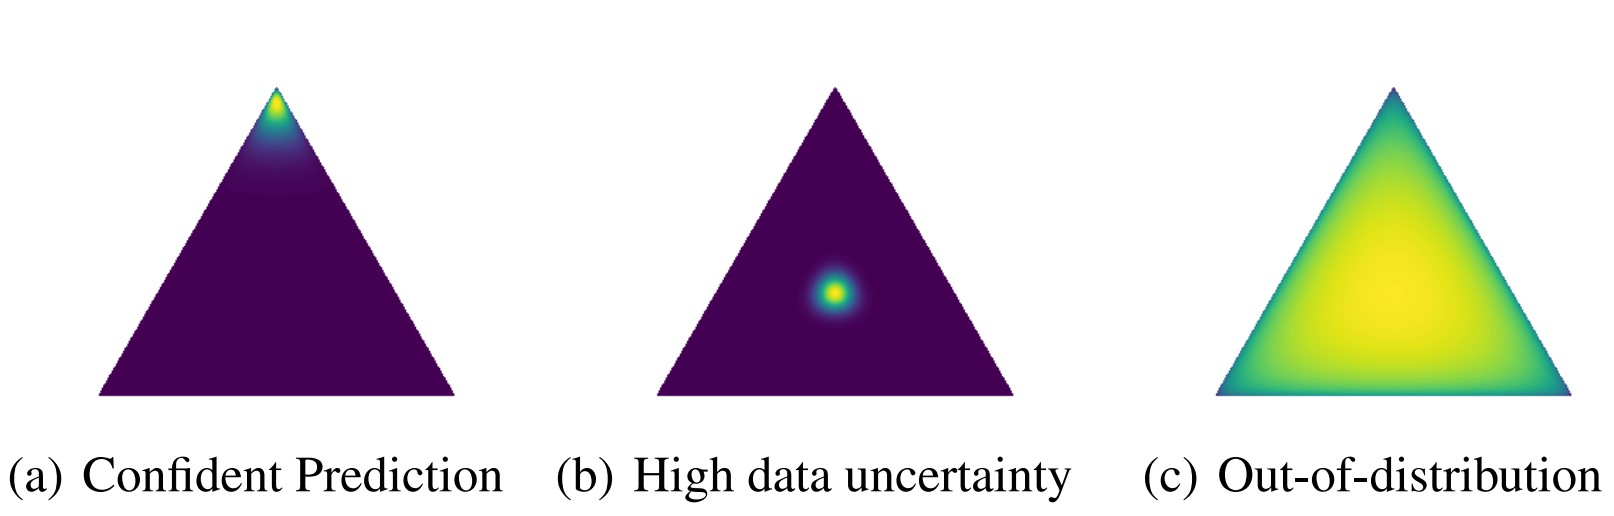
\includegraphics[scale=0.25]{examples.jpg}
     \end{figure}
\end{frame}
\begin{frame}{Dirichlet Prior Networks}
    Considering marginalization of $\theta$ in last equation:
    $$\int p(\omega_c | \mathbf{\mu}) \int \left[ p(\mu | \mathbf{x}^*, \mathbf{\theta})p(\mathbf{\theta}|D) d\mathbf{\theta} \right] d\mathbf{\mu} = \int p(\omega_c | \mathbf{\mu}) p(\mu | \mathbf{x}^*, D)$$
    So, the loss function:
    $$L(\mathbf{\theta}) = \mathbb{E}_{p_{in}(x)}[KL[Dir(\mathbf{\mu} | \mathbf{\hat{\alpha}}) || p(\mu | \mathbf{x}, \mathbf{\theta})]] + \mathbb{E}_{p_{out}(x)}[KL[Dir(\mathbf{\mu} | \mathbf{\tilde{\alpha}}) || p(\mu | \mathbf{x}, \mathbf{\theta})]]$$
    where $\mathbf{\hat{\alpha}}$ - in-distribution targets,
    $\mathbf{\tilde{\alpha}}$ - out-of-distribution targets.
\end{frame}

\begin{frame}{Uncertainty Measures}

\begin{enumerate}
    \item Max probability:
        $$P = max_c P(\omega_c | \mathbf{x}^*, D)$$
    \item Entropy:
        $$H[P(y | \mathbf{x}^*, D)] = - \sum_{c=1}^KP(\omega_c | \mathbf{x}^*, D) \ln(P(\omega_c | \mathbf{x}^*, D))$$
    \item Mutual Information between $y$ and $\theta$ (MI):
         $$I[P(y, \theta | \mathbf{x}^*, D)] = H[E_{p(\theta|D)}P(y | \mathbf{x}^*, \theta)] - E_{p(\theta|D)}H[P(y | \mathbf{x}^*, \theta)]$$
    \item Mutual Information between $y$ and $\mu$ (MI):
        $$I[P(y, \mu | \mathbf{x}^*, D)] = H[E_{p(\mu|\mathbf{x}^*,D)}P(y | \mu)] - E_{p(\mu|\mathbf{x}^*,D)}H[P(y | \mu)]$$
    \item Differential entropy:
        $$H[p(\mu | \mathbf{x}^*, D)] = - \int_{S^{K-1}}p(\mu | \mathbf{x}^*, D) \ln p(\mu | \mathbf{x}^*, D)d\mu$$
\end{enumerate}
\end{frame}
\begin{frame}{Synthetic experiments}
    \begin{figure}[h]
        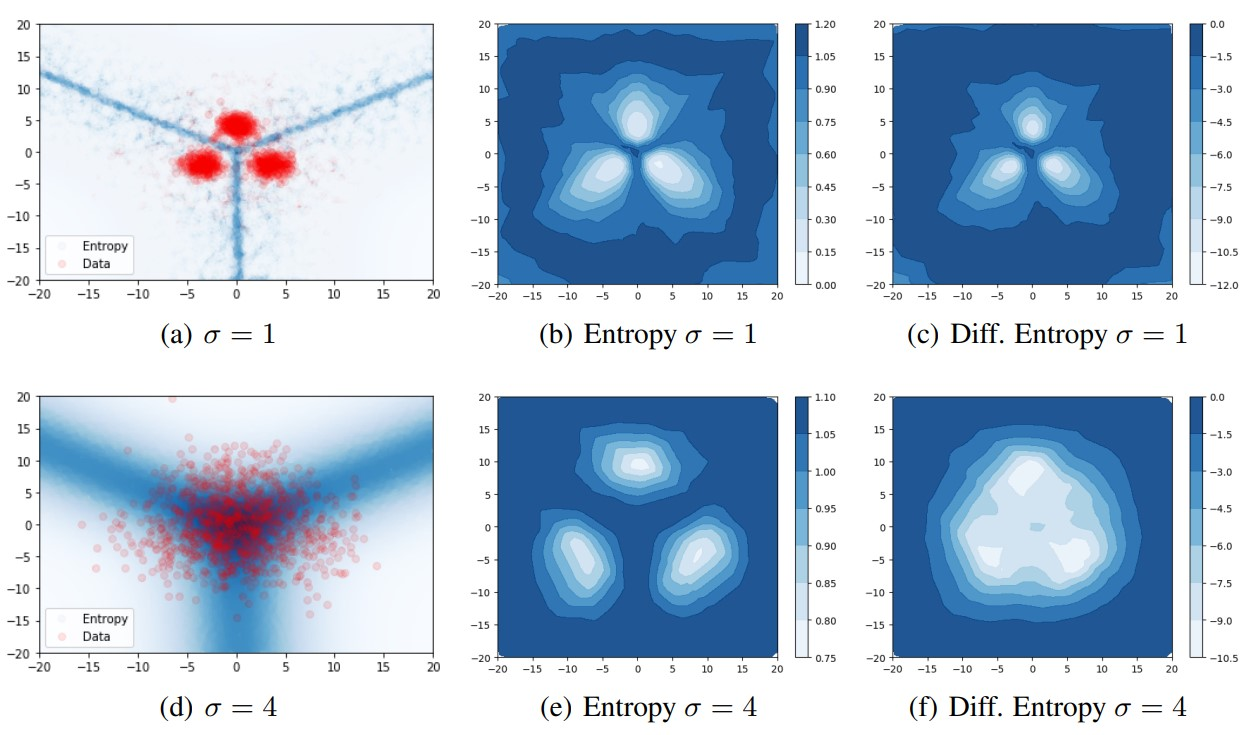
\includegraphics[scale=0.3]{results.jpg}
     \end{figure}
\end{frame}

\begin{frame}{MNIST and CIFAR-10 experiments}
    \begin{figure}[h]
        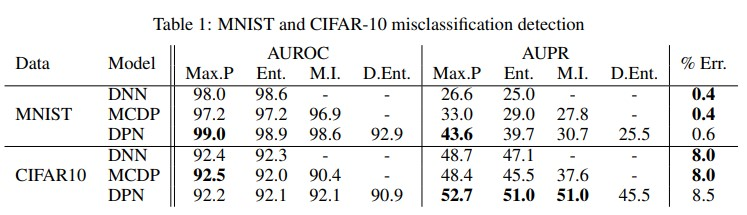
\includegraphics[scale=0.6]{images/table1.jpg}
     \end{figure}
\end{frame}

\begin{frame}{MNIST and CIFAR-10 experiments}
    \begin{figure}[h]
        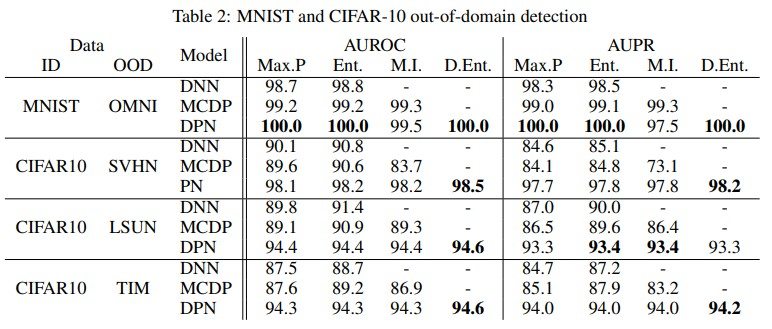
\includegraphics[scale=0.5]{images/table2.jpg}
     \end{figure}
    \begin{figure}[h]
        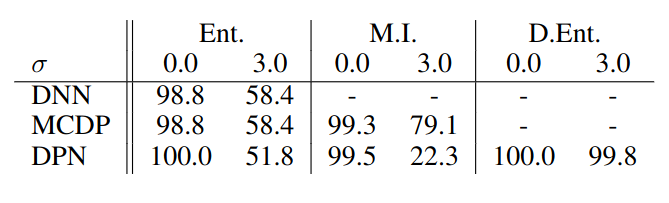
\includegraphics[scale=0.35]{images/table3.png}
     \end{figure}
\end{frame}

\end{document}
